
\section{Introduction to Language Modeling}
\label{sec:language-modeling}

Language modelling is has the goal of determining a probability distribution on sequences of words (like sentences).
A (statistical) language model estimates a function which calculates the probability $p$ for the word sequence $w_1,\dots,w_m$:
\[
    p(w_1,\dots,w_m) = \prod_{i=1}^{m} p(w_i | w_1,\dots,w_{i-1})
\]
The fundamental challenge here is the dimensionality and vocabulary size of the data. For example to model the joint distribution
of 10 word sequences with a vocabulary $V$ size of 100.000 there are potentially $100000^{10} - 1$ 
free parameters~\cite{Bengio:2003:NPL:944919.944966}. 

% ==========================================================================================
\subsection{N-Gram Models}
\label{subsec:n-gram}

An n-gram is a contiguous sequence of n items / words from a given sequence of text or speech. Compared to the language model above,
we only try to estimate a probability distribution for the last $n$ words out of the sequence, we approximate the actual language model:
\[
p(w_1,\dots,w_m) = \prod_{i=1}^{m} p(w_i | w_1,\dots,w_{i-1}) \approx \prod_{i=1}^{m} p(w_i | w_{i-(n-1)},\dots,w_{i-1})
\]

So we assume we can approximate the probability for $w_i$ by replacing the context of the preceding $i - 1$ words with 
the context of the previous $n - 1$ words. Formally this is a $n - 1$ order Markov chain. % TODO citation, is it n or n-1 order?

For a 1-gram sequence this is called an unigram, a 2-gram s a bigram, n = 3 is a trigram and so forth.
One could estimate the conditional probabilities by counting all occurrences in the sample data:
\[
p(w_i\mid w_{i-(n-1)},\ldots,w_{i-1}) = \frac{\mathrm{count}(w_{i-(n-1)},\ldots,w_{i-1},w_i)}{\mathrm{count}(w_{i-(n-1)},\ldots,w_{i-1})}
\]
Of course this is very impractical, the number of possible sentences is too big. Additionally a training sample probably 
won't contain all possible combinations and therefore it's not possible to calculate estimations for all of them in this way.
In the next section we are going into some techniques used to mitigate this.

\subsubsection{Smoothing Techniques}

We need to be able to estimate word combinations wich we have previously not seen and assign a non-zero probability to them.
Some form of smoothing is necessary, the simplest possible solution is to just "add-one" to every word count.
This is called "Laplacian smoothing" and allows us to assume a count of 1 for unseen n-gram's. 

A better way is to use less context in these situations and to "Backoff". For example use a trigram instead of a 4-gram or a bigram and so on.
Additionally it can be a good solutions to mix results from unigram, bigram, trigram etc and linearly interpolate between them.
A more sophisticated way is to use neural networks, which represent words in a distributed way as 
a non-linear combinations of weights in a graph \cite{Hinton:1986:DR:104279.104287}.


% ==========================================================================================
\subsection{Perplexity}
\label{subsec:perplexity}

As we have previously seen, language modeling amounts to learning a posteriori probability distribution. 
Perplexity is a measure of how well a probability distribution predicts sample data. It can be 
interpreted as the number of choices per word position.
We can use it to formally judge how well a language model can predict the distribution. The exponent in the Perplexity term below
is the Entropy, it expresses the number of bits required to represent an event (in our case a word or character).

Formally Perplexity is defined as the sum of the inverse log-probabilities
\[
    2^{H(p)}=2^{-\sum_x p(x)\log_2 p(x)}
\]
Where $H(p)$ is the entropy~\cite{Shannon:1948} of the probability 
distribution $X$ of values ${x_1,\dots,x_n}$ with the probability mass function $p: X \rightarrow [0,1]$.

To minimize the perplexity value means to have a better fitting language model.

\subsubsection{Entropy}

Shannon~\cite{Shannon:1948} or Bit-Entropy is defined as $log_2(n)$ where $n$ is the number of possible outcomes. 
This assumes that all possible outcomes have the same probability. For a probability distribution 
we need to consider all three possible values ${x_1,\dots,x_n}$ it's likelihood of appearance and the entropy every possible outcome has.

The entropy of a value $x_i$ is dependent on it's self-information, which is inversely proportional to it's probability:
$I(x_i) = log(\frac{1}{p(x_i)}) = -log(p(x_i))$.
The self information of an intersection of two independent events $A$, $B$ is the sum of both: $I(A \cap B) = I(A) + I(B)$.
This is why the $log$ function is used to wrap $\frac{1}{p(x_i)}$.
In total the entropy for $X$ is defined as the expected information content of $X$: 
\[
    H(p) = E(I(X)) = -\sum_{i=1}^{n} p(x_i)\log_2 p(x_i)
\]

% ==========================================================================================
%\subsection{Skip-N-Gram Models}
% Possible cut depending on how the rest turns out

% The trouble with n-gram style language models is that they only consider the previous $n-1$ words regardless whether they have any real
% impact on the next word or not. The idea with the skip-n-gram model is to allow for a flexible context, which does not have to be
% the directly preceding words.
% \cite{DBLP:journals/corr/abs-1301-3781}


% ==========================================================================================
\subsection{Continuous space language models}
\label{subsec:cslm}

Continuous space language models can base their predictions on continuous representations of words. The word embeddings, which we will
discuss further in section~\ref{sec:c2w}, are a way to represent words in a continuous vector space. 
Continuous space embeddings help to alleviate the curse of dimensionality in language modeling, which arises out of the larger 
training texts. By representing the words in neural networks in a distributed way, 
we no longer have such a big issue with previously unseen word variations.

As with the simple counting based model from~\ref{subsec:n-gram} the neural network continuous space language models train to
estimate a probability distribution for the word $w_i$ given the linguistic context.
\[
    p(w_i|\text{context}) \forall w_i \in V
\]
As with the n-gram models the context can be for example limited to a fixed number of previous words. In contrast to the
simple counting model, a neural network can learn the complex non-local relationships between the word types in sequences.

\subsubsection{Classical Neural Language Model}

The classical neural language model architecture performs two tasks: First it projects the input words into the continuous vector space,
secondly it computes the language model probability for the given context. These task can be performed by two 
hidden layers~\cite{Schwenk:2007:CSL:1230156.1230409}. 
First every input word $w_i$ is encoded into vectors $1_{w_i}$ where
the entry corresponding to the index of $w_i$ within the vocabulary $V$ is $1$ and all other entries are $0$. 
This is then multiplied with a projection matrix $P \in \mathbb{R}^{|V| \times d}$ where $d$ is the dimension of the embeddings.
The embedding is obtained from $P$ by multiplying with a selection vector $1_{w_i}$, 
which is 1 at the word index: $e_{w_i}^W = P * 1_{w_i}$. The matrix $P$ is basically a lookup 
table for the word embeddings. 
The projections of all words in the context of the previous $n-1$ words are concatenated and form 
the first hidden layer (called the projection layer) of the NNLM.

A NNLM will always compute the probability for \textit{all} words contained in the vocabulary $V$. 
This is performed in combination by the second hidden layer and the output layer. 
The hidden layer will compute $d_j = f(\sum_{l = i-n+1}^{i-1} e_{w_l} * m_{lj} + b_l) \forall j = 1 \dots H$, 
where $H$ is the number of hidden neurons, $m_{lj}$ are the weights between the projection layer and the second hidden layer,
$b_j$ is the activation bias of neuron $j$. This combines all the word embeddings $e_w$ into an $H$ dimensional representation.
In the output layer this has to be scaled up to the vocabulary size again, 
by computing $z_k = \sum_{j = 1}^{H} v_{kj} * d_j + b_k \forall k = 1 \dots |V|$, where $v_{kj}$ are the weights of the output layer.
Since we have to transform this into a valid probability, the output layer uses a softmax function 
(introduced in section~\ref{subsec:softmax}), which will finally convert all $z_k$ values into probabilities $p_k$.
 
\begin{figure}[H]
\begin{center}
  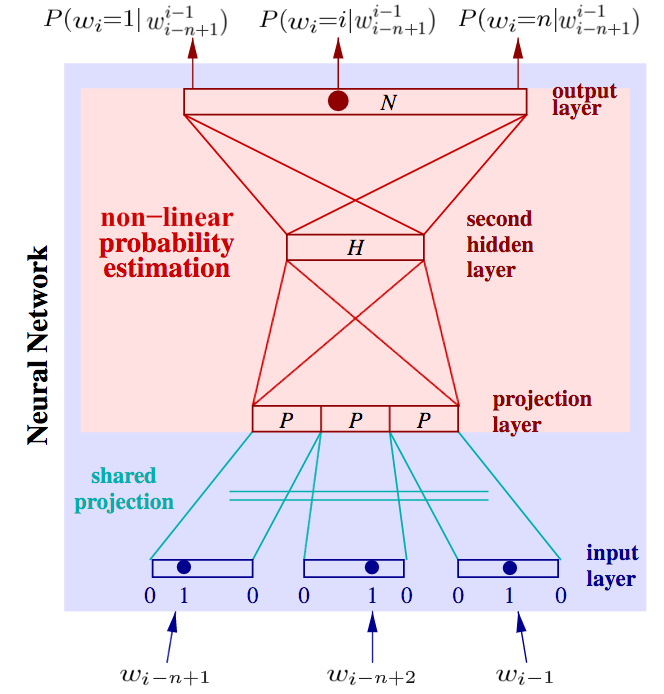
\includegraphics[width=0.7\textwidth]{./img/classic_nnlm}
  \caption{Architecture of a neural network language model, the context is denoted as $w_{i-n+1}^{i-1} = w_{i-(n-1)},\dots,w_{i-1}$.
  The output layer is a softmax over the vocabulary.
  (Figure taken from~\cite{Schwenk:2007:CSL:1230156.1230409}).}
  \label{fig:classic_nnlm}
\end{center}
\end{figure}

After training the resulting vector representations stored in $P$ can then be reused in other tasks.
This has the advantage that tasks with low amounts of training data can be trained together with tasks with larger amounts of data.
In section~\ref{subsec:language-model-c2w} we are going to discuss how to apply the word embeddings from section~\ref{sec:c2w} in
a neural natural language model, which is going to be structurally similar to the one presented here.

\subsubsection{Softmax Layer}
\label{subsec:softmax}

The Softmax function is a \textit{logistics function} and is often used as the final combining processing layer in neural
networks. It calculates a normalized exponential that 'squashes' the input such that the resulting vector entries add up to 1.
\[
    p_k = \sigma(\mathbf{z})_k = \frac{e^{z_k}}{\sum_{k=1}^{|V|} e^{z_k}}
\]
\begin{figure}[H]
\begin{center}
  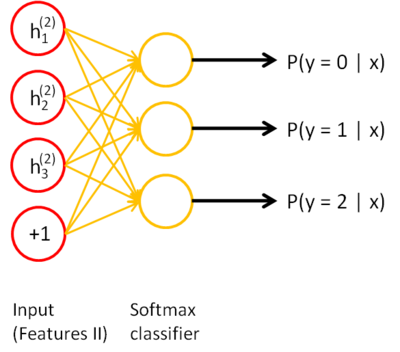
\includegraphics[width=0.5\textwidth]{./img/softmax_layer}
  \caption{Structure of a softmax layer in a neural network}
  \label{fig:softmax_layer}
\end{center}
\end{figure}

The property of the softmax layer is that the result of the outputs can be interpreted as posterior probabilities. 
This is useful in classification as it gives a valid posteriori propability measure for an n-gram model.
A softmax layer transforms the results of a hidden layer into a probability distribution for neural language models. The NNLM assigns the
probability given the context: $p_k = p(w_i = k | w_{i-n+1}^{i-1})$.

\subsubsection{Out of Vocabulary Token}

Since the softmax can only be computed for known words included in the vocabulary set $V$ it is not possible to handle words
not included in $V$ during testing.
These words are \textbf{Out Of Vocabulary} (OOV), the solution is to replace all of them with an special token word.
The probability for this OOV token can be learned during the training stage, by replacing word types with low frequencies with the $<$OOV$>$ token.
During test time we can now use the $<$OOV$>$ probabilities for any word not in the vocabulary $V$~\cite{DBLP:journals/corr/LingLMAADBT15}.

For a language modeling task where there is not a closed Vocabulary, we will almost certainly encounter words which are not known from
our training vocabulary set. It is therefore essential to apply a strategy like the above one to have a robust estimation
for OOV words.

